% !TEX ROOT = ersti.tex
\setboolean{druckversion}{false}
\newcommand{\altstadtkarte}{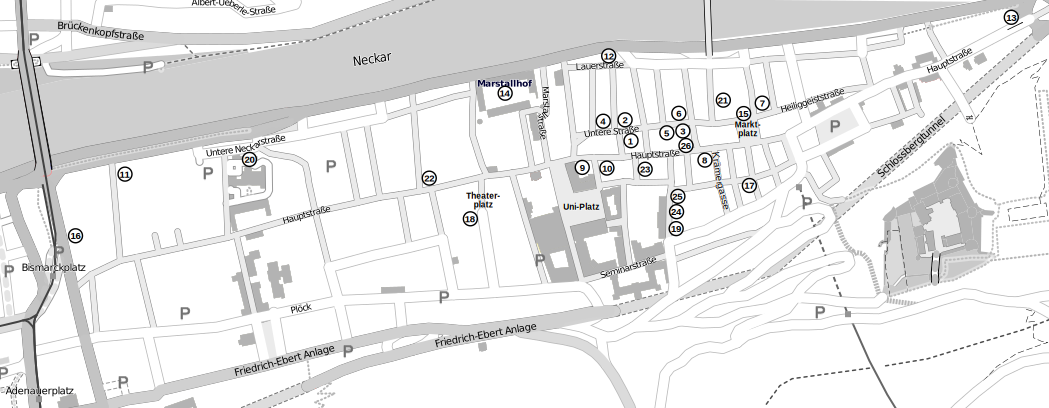
\includegraphics[width=\textwidth, trim=10mm 0mm 80mm 0mm, clip]{bilder/altstadt.pdf}} % Vektor
\newcommand{\coverimage}{cover/ErstiInfo_Cover_2024_Vorderseite.png}
\newcommand{\festimage}{cover/ErstiInfo_Cover_2024_Rueckseite.png} %Rückseite, da war früher mal das Festplakat
\newcommand{\nhfkarte}{cover/nhf_rgb.pdf}
\newcommand{\philwegkarte}{cover/philweg_rgb.pdf}
\usepackage[pdftex,bookmarks=true,bookmarksnumbered=true,colorlinks=true,filecolor=black,linkcolor=red,urlcolor=blue,plainpages=false,pdfpagelabels,citecolor=black]{hyperref} % Für tolle Verlinkungen

% RGB Farben für's Web sind hinreichend gut. Sonderfarben machen das PDF
% ca. 1.5 MB größer
\definecolor{kapitelhintergrund}{RGB}{101,168,101}
\definecolor{sectiontextfarbe}{RGB}{38,100,38}

\usepackage[columnsep=10mm, outer=25mm, bottom=30mm, top=30mm]{geometry} % für ein passendere Layout

% Trim options
\showtrimsoff
